
\begin{figure}[b]%
\centering
\parbox{2.0in}{

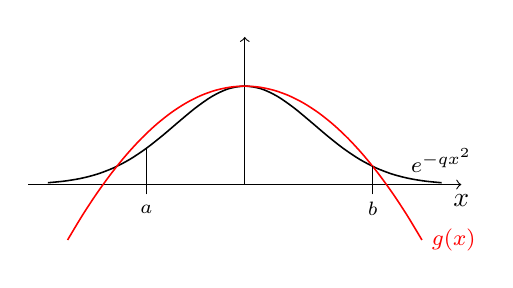
\begin{tikzpicture}[scale=1.25]
\draw[->] (-2.2,0) -- (2.2,0) node[anchor=north] {$x$};
\draw[->] (0,0) -- (0,1.5) node[anchor=east] {};
\draw[smooth, domain=-2.0:2.0, color=black, line width=0.20mm] 
    plot (\x,{e^(-(\x*\x))}) node [above] {\footnotesize $e^{-qx^2}$};
\draw[smooth, domain=-1.8:1.8, color=red, line width=0.20mm] 
    plot (\x,{-0.4825*\x*\x+1}) node [right] {\footnotesize $g(x)$};
\draw (1.3,-0.1) -- (1.3,{e^(-1.3*1.3)});
\draw (-1,-0.1) -- (-1,{e^(-1*1)});
\draw	(-1,-0.25) node{{\scriptsize $a$}}
		(1.3,-0.25) node{{\scriptsize $b$}};
\end{tikzpicture}

%\caption{A parabola over a gaussian curve}%
\label{fig:graph111}
}
\end{figure}
